\section{General Data Management Policies}
\label{sec:relation-to-load-balancing}

%\begin{itemize}
%  \item Lustre Trace
%  \item LinkedIn Trace
%  \item Nathan's Trace
%\end{itemize}

In the previous section, we used our data management language and the Mantle
policy engine to design effective cache management strategies for a new service
and domain. In this section, we compare and contrast the policies examined for
file system metadata load balancing in~\cite{sevilla:sc15-mantle} with the ones
designed for cache management in ParSplice. The similarities show how the
``when"/``where"/``how much" abstractions, data management language, and policy
engine may be widely applicable to other data management techniques, such as
QoS, scheduling, and batching.

\subsection{Using File System Policies for ParSplice}
%- memory utilization/heuristics
From a high-level the ParSplice policy trims the cache if the cache reaches a
certain size {\it and} if it has already absorbed the initial burstiness of the
workload; the CephFS poicy, which is shown in Figure~\ref{src:lua-cephfs},
migrates load if the metadata load is higher than the average load {\it and}
the current load has been overloaded for more than two iterations.

\textbf{Condition for ``Overloaded"} (Fig.~\ref{src:lru-dyn}: Line 2;
Fig.~\ref{src:lua-cephfs}: Line 2) - these lines detect whether the node is
overloaded using the ``load" calculated in the load callback; while the load
calculations and thresholds are different, the actual logic is exactly the
same.  Recall that this decision is made locally because there is no global
scheduler or centralized intelligence. 

\textbf{State Persisted Across Decisions} (Fig.~\ref{src:lru-dyn}: Lines 4,6;
Fig~\ref{src:lua-cephfs}: Lines 3,4,10) - these lines use Mantle to write/read state
from previous decisions.  For ParSplice, we save a boolean that indicates
whether we have absorbed the workload's initial burstiness. For CephFS, we save
the number of consecutive instances that the server has been overloaded. We
also clear the count (Line 10) if the server is no longer overloaded. The
underlying implementation saves the values to local disk.

\textbf{Condition that Switches Policy} (Fig.~\ref{src:lru-dyn}: Line 6;
Fig.~\ref{src:lua-cephfs}: Line 5) - these lines switch the policies using
information from previous decisions. ParSplice trims its cache once it eclipses
the ``absorb" threshold while CephFS allows balancing when overloaded for more
than two iterations. The persistent state is essential for both of these
policy-switching conditions.

\begin{figure}[t]
\footnotesize
\begin{minted}[xleftmargin=3em,linenos]{lua}
local function when()
  if servers[whoami]["load"] > target then
    overloaded = RDstate() + 1
    WRstate(overloaded)
    if overloaded > 2 then
      return true
    end
  end
  else then
    WRstate(0)
  end
  return false
end
\end{minted}
\caption{CephFS file system metadata load balancer.\label{src:lua-cephfs}}
\end{figure}

\subsection{Using ParSplice Policies for File Systems}

%- how many inodes to keep in mds/client caches
%- affects LB; increases capacity of single MDS (reduces req/mem pressure)
%- affects LB; tells us which part of the cache to keep local

% Load balancing in FSs
Mantle was designed for file system metadata load balancing across a cluster of
dedicated metadata servers, where spreading requests across servers improves
performance. But another technique to reduce request load is to keep caches on
both clients and servers. The caches in CephFS have the same performance and
utilization trade-off as ParSplice, where large caches improve performance at
the expense of a large memory footprint. High memory utilization is problematic
when a single metadata server services many clients with their own caches.
Using cache management policies has two benefits for load balancing: (1)
increases the capacity of a single metadata server, and (2) helps identify
which parts of the cache to keep local to a server. Applying the regime
detection algorithm from Section~\S\ref{sec:regime-detection} to a similar file
system access pattern has the potential to identify when to migrate keys and
how many keys to migrate.

% burstiness of creates then compile
To show how regime detection helps load balance file system metadata across a
cluster, consider the trace of metadata requests for compiling a large project
in CephFS shown in Figure~\ref{fig:compile-ops}. That trace shows the number of
file system metadata requests serviced by the metadata server when
uncompressing (\texttt{untar}), compiling (\texttt{make}), and deleting
(\texttt{rm}) the source code for the Linux kernel. If the system knows that
the job phases would progress from many creates, to many lookups, to many
deletes, then it could size its caches accordingly. For example, the file
system could cache none of the inodes from the \texttt{untar} phase and run
regime detection during the \texttt{make} phase and only cache the inodes that
are repeatedly used. This will be less than 20K inodes and could result in up
xMB in memory footprint savings without sacrificing performance.

%- strategy: cache all inodes on create
\begin{figure}[t]
  \noindent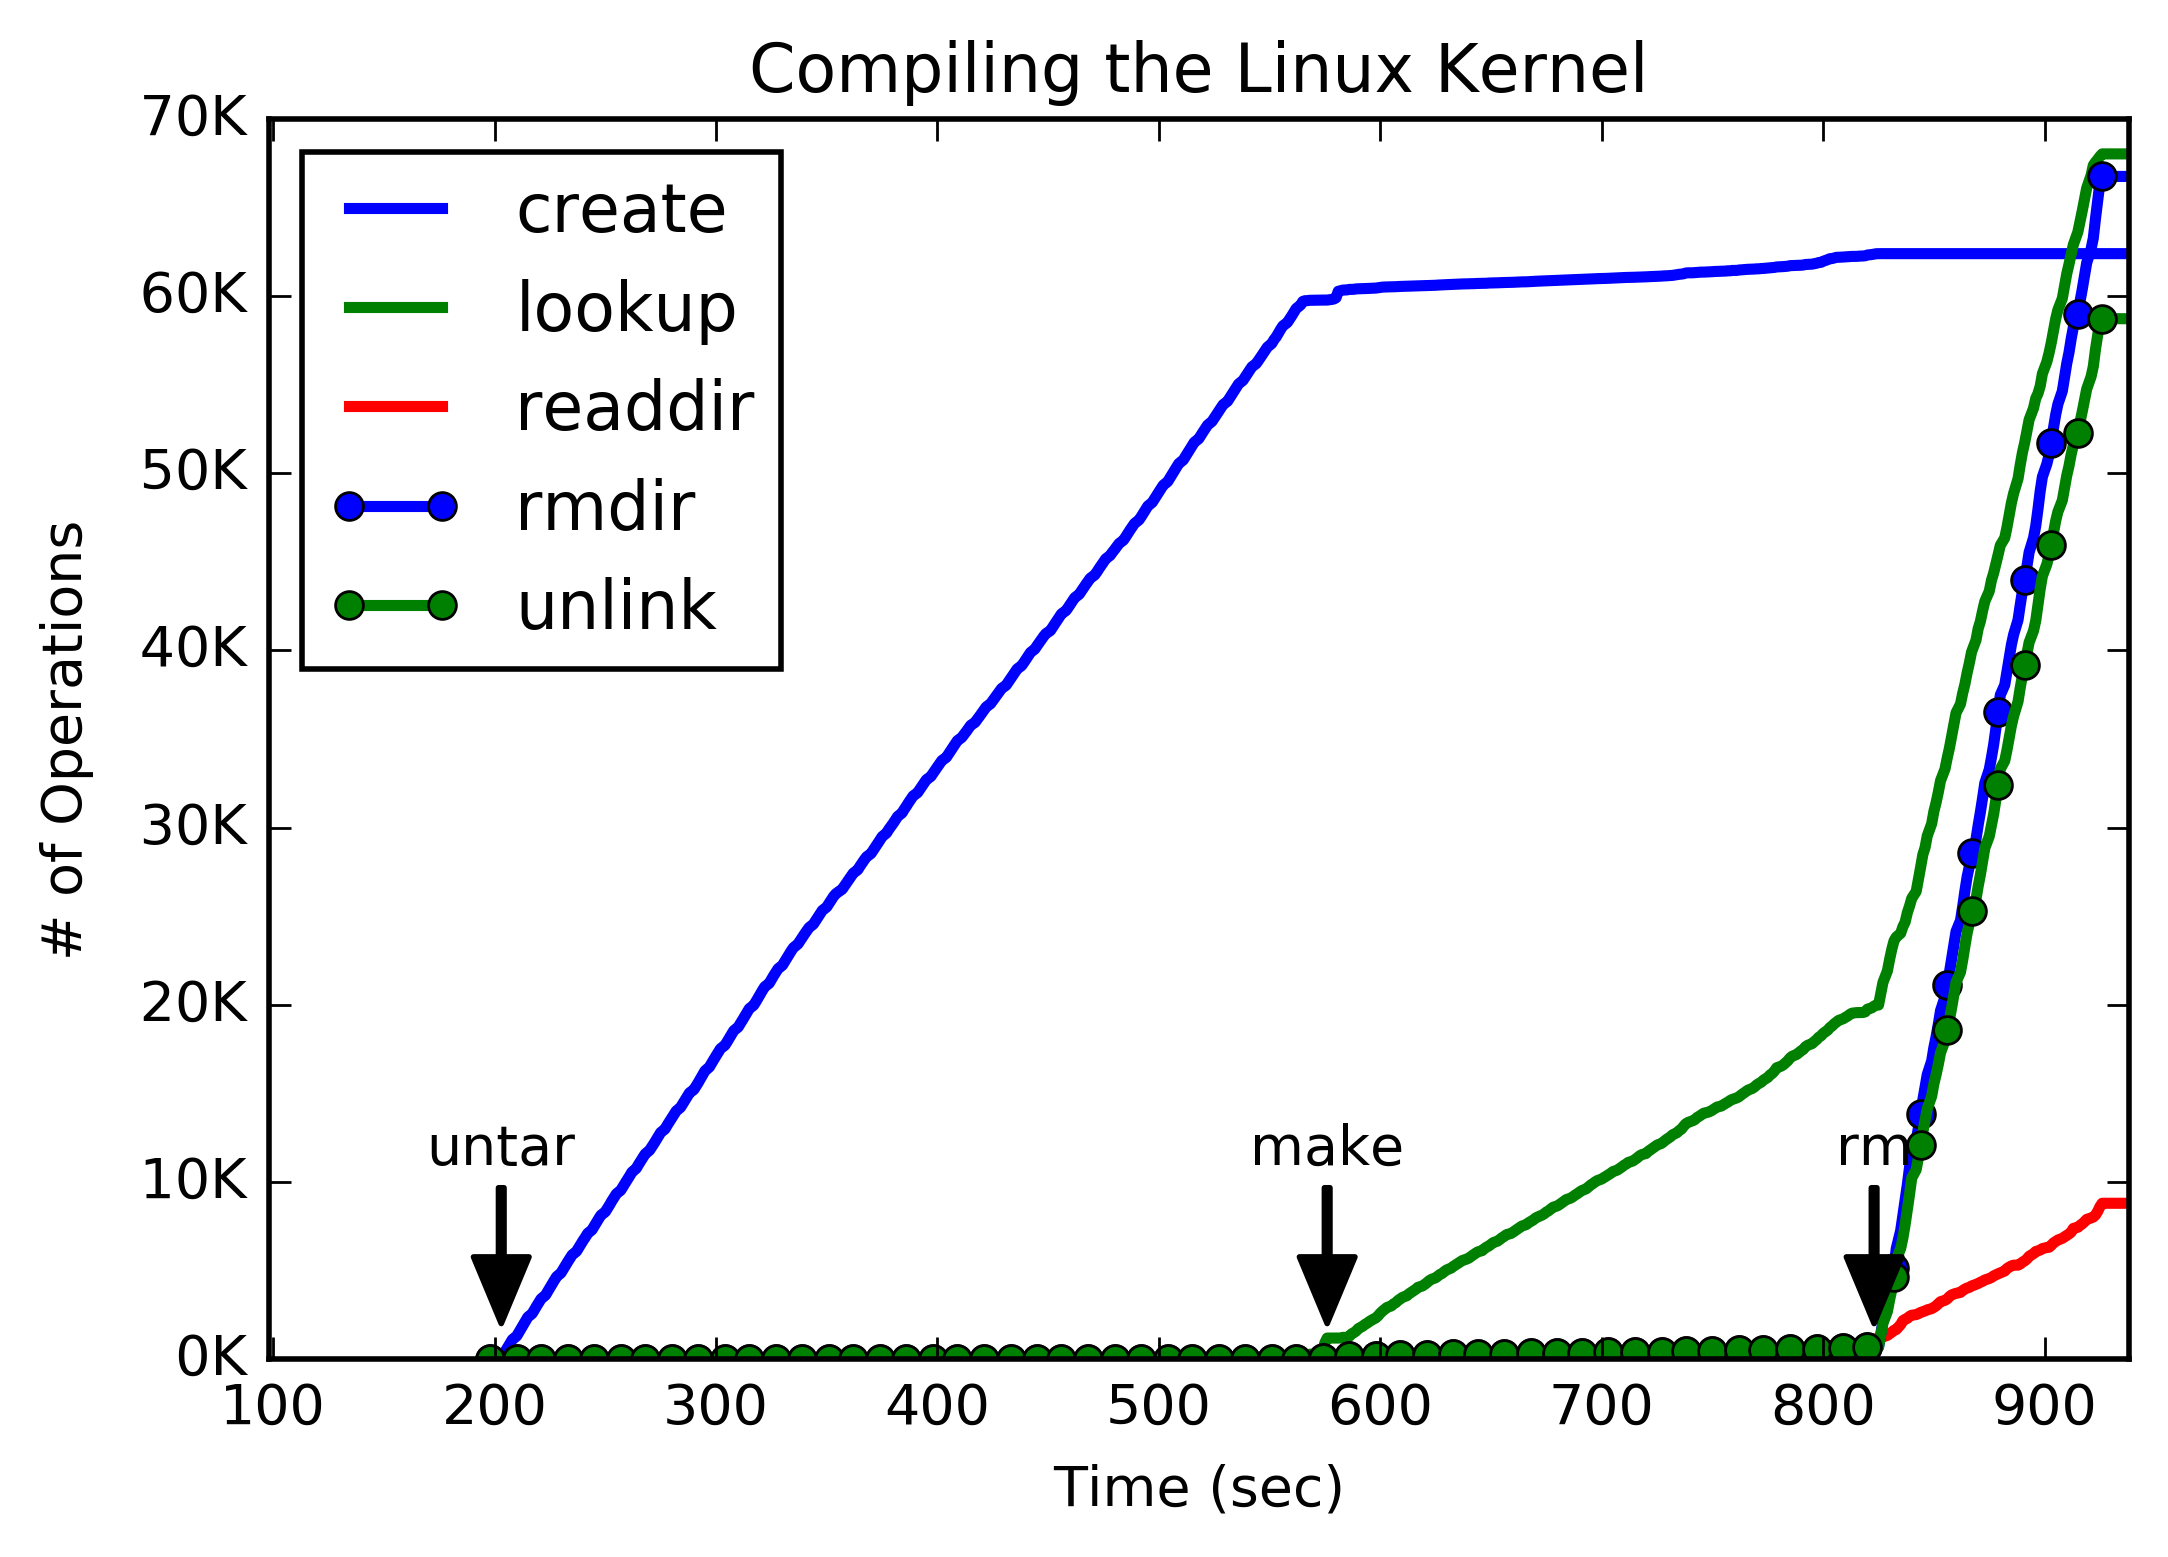
\includegraphics[width=0.5\textwidth]{figures/compile-ops.png}\\
\caption{ \label{fig:compile-ops}} \end{figure}

% other use cases caches/tiers 
Ceph has many other data management techniques that would benefit from the
caching policies developed in
Sections~\S\ref{sec:cache-management-using-system-archiecture-knowledge}
and~\ref{sec:cache-management-using-domain-specific-knowledge}. Administrators
can use the policies in ParSplice to automatically size and manage cache tiers
\footnote{http://docs.ceph.com/docs/master/rados/operations/cache-tiering/}, caching on
object storage devices, or in the distributed block
devices\footnote{http://docs.ceph.com/docs/master/rbd/rbd-config-ref/}.
Integration with Mantle would be straightforward as it is merged into Ceph's
mainline\footnote{http://docs.ceph.com/docs/master/cephfs/mantle/} and the
three caching subsystems mentioned above already maintain keyspace access
traces. We hypothesize that since this is all software defined caching,
something more clever than LRU would improve cache utilization and performance.

http://docs.ceph.com/docs/master/dev/mds_internals/data-structures/

\subsection{Other Use Cases}
% we said this is good for LB/Cache management... what about others??
% QoS: when to move clients, where to move clients, how much of the reservation to move
% Other cache management: MRU
% Scheduling: how much of a resource to allocate; more than just LRU (RAD)
%\subsection{Visualizing File System Traces like ParSplice Keyspace Traces}

